 \chapter{高维几何,Johnson-Lindenstrauss引理}\label{chap:J-L-Lemma}

作为生活在三维空间中的人,一个令我们倍感着迷的问题是:如果我们的世界是四维、五维甚至更高维的,我们会看到什么样的景象?Christopher Nolan导演的电影《星际穿越》(Interstellar)给出了一个美妙的想象. 

在近未来的地球上,资源匮乏和环境恶化使人类濒临灭绝. 为了寻找新的生存空间,一群科学家和宇航员开始了一次前所未有的宇宙冒险. 他们的目标是穿越一个神秘的虫洞,探索另一片星系中的适居行星. 

然而,当主人公Cooper和他的团队成功穿越虫洞时,他们发现自己面对的并不仅仅是遥远的星系,还有更加不可思议的挑战. 在探索的过程中,Cooper最终进入了一个被称为tesseract的空间——一个超越我们三维世界的五维空间. 在这个空间中,时间变得像空间一样可以自由导航,过去和未来不再是固定不变的线性进程,而是可以被观察和影响的维度. 

通过操控时间维度,库珀能够在这个超立方体般的结构中,跨越时间的界限,影响他女儿Murph的命运,从而拯救全人类. 这一情节不仅带给我们震撼的视觉体验,也揭示了一个深刻的物理与几何真理:在高维空间中,我们的直觉常常失效,必须依赖数学工具来理解和探索这些新维度的性质. 

高维空间不仅是科学幻想中的概念,也是现实中的客观存在:当我们描述一个人的时候,我们会考虑他的年龄、身高、体重、学历、职业等多个属性,这些属性构成了一个多维的空间. 在这个空间中,每个人都是一个点,而这些点之间的距离和关系,构成了我们对这个人的认知和理解. 

在计算机的世界中,世界的一切都被表示为了数据,而且往往是高维数据. 因此,如何理解和处理高维数据已经成为人工智能领域的一个重要问题. 

本章将说明,高维空间有着令人着迷却看似矛盾的两种性质. 首先,与我们生活的三维空间相比,高维空间是极其反直觉的,这带来了望而生畏的复杂性,似乎“维数灾难”难以逾越. 然而,硬币的另一面是,高维空间中的随机数据几乎都是高度集中,因而他们其实可以被压缩到更低维度的空间中进行处理. 这一原理被广泛应用在机器学习中. 

从技术上看,我们要证明Johnson-Lindenstrauss引理,它表明了高维随机变量的集中性. 证明这一引理所用到的概率论技术是\textbf{矩法},这是\textit{机器学习理论}中最为核心的几个技术之一. 因此本章也可以看做机器学习理论的一个引论. 

\section{高维几何}

\subsection{高维球体}
首先,我们探讨高维空间中“球体”的特殊性. 按照微积分的方式(见\Cref{subsec:kolmogorov-probability}),我们可以定义$n$维空间中的体积和表面积. 定义
\[B_n = \{x \in \R^n: \norm{x} \leq 1\}.\]
这是一个$n$维空间中的单位球体. 

第一个反直觉的事实是,随着$n$趋于无穷,$B_n$的体积和表面积都会趋于零!首先,我们给出$n$维单位球体的体积和表面积的计算公式:

\begin{theorem}\label{thm:volume-surface-area}
记$V_n$为$n$维单位球体的体积,$S_n$为$n$维单位球体的表面积. 那么,
\begin{align*}
    V_n&=\frac{\pi^{n/2}}{\Gamma(1+n/2)},\\
    S_n&=\frac{2\pi^{n/2}}{\Gamma(n/2)}.
\end{align*}
其中$\Gamma$是Gamma函数,对自然数$n$,它定义为
\[\Gamma\left(\frac{n}{2}\right)=\begin{cases}
    (m-1)!, & n=2m,\\
    \frac{(2m)!}{4^mm!}\sqrt{\pi}, & n=2m+1.
\end{cases}
\]
\end{theorem}
这一定理的证明对积分的技巧要求较高,我们这里不给出,感兴趣的读者见习题 \ref{exercise:volume-surface-area}.

这一定理的推论是,随着$n$的增大,$V_n$和$S_n$都会趋于零:

\begin{corollary}
\begin{align*}
    \lim_{n\to\infty} V_n&=0,\\
    \lim_{n\to\infty} S_n&=0.
\end{align*}
\end{corollary}
\begin{proof}
    当$n$趋于无穷时,由Stirling公式,我们有
        \[\Gamma(n)\sim\sqrt{2\pi n}\left(\frac{n}{e}\right)^n.\]
    因此,当$n\to\infty$,
    \[V_n\sim\frac{\pi^{n/2}}{\sqrt{2\pi n}\left(\frac{n}{e}\right)^n}=\frac{1}{\sqrt{2\pi n}}\left(\frac{e}{n\sqrt{\pi}}\right)^n\to 0.\]
    同理,$S_n$的极限也为$0$.
\end{proof}

接下来,我们说明,高维空间中的球体质量分布是极其不均匀的,大部分质量都集中在球体的边界上. 定义一个半径为$r$的$n$维球为
\[B_n(r) = \{x \in \R^n: \norm{x} \leq r\}.\]
那么我们有:
\begin{proposition}
对任意$\epsilon\in(0,1)$,
\[\frac{\lambda(B_n(1-\epsilon))}{\lambda(B_n(1))}=(1-\epsilon)^n.\]
其中$\lambda$是$\R^n$上的Lebesgue测度(体积). 

因此,当$n$趋于无穷时,这一比值以指数速度趋于零. 
\end{proposition}
\begin{proof}
    利用体积(Lebesgue测度)的性质(见\Cref{subsec:kolmogorov-probability}),
    \[\lambda(B_n(r))=r^n\lambda(B_n(1)).\]
    代入$r=1-\epsilon$,即可得证.
\end{proof}

接下来,我们再说明,如果把$n$维球和$n$维超立方体放在一起看,他们的质量分布也是非常反直觉的. 对于$n \in \N$,$\epsilon>0$,定义我们定义一个$n$维的“球壳”$A_{n,\epsilon}$:

\[A_{n,\epsilon} = \{x \in \R^n:(1-\epsilon)\sqrt{n/3}<\norm{x}<(1+\epsilon)\sqrt{n/3}\}.\]
这是一个半径为$\sqrt{n/3}$的$n$维“球壳”,厚度为$2\epsilon$. 

我们有如下定理:
\begin{theorem}
\[\lim_{n\to \infty} \frac{\lambda (A_{n,\epsilon}\cap (-1,1)^n)}{\lambda((-1,1)^n)} = 1,\]
其中$\lambda$是$\R^n$上的Lebesgue测度(体积). 
\end{theorem}

我们来解释这一定理反直觉的地方. 
\begin{itemize}
    \item 如果我们只看方向$(1,0,\dots,0)$(或者其他“正方向”),半径为$\sqrt{n/3}$的球壳应该远远超出了$(-1,1)$的范围. 然而,这一定理告诉我们,球壳在超立方体内占据了几乎全部的体积,这说明在其他的方向,球体以不可思议的方式被“压扁”了. 
    \item 当$n$很大时,超立方体$(-1,1)^n$的绝大部分体积都是由一个厚度为$\epsilon$,半径为$\sqrt{n/3}$的$n$维球壳提供的,当$\epsilon$很小时,这个球壳非常薄. 一层\textit{薄}球壳占据了一个\textit{实心}立方体的绝大部分体积,这个在二维和三维空间中也是难以想象的. 
\end{itemize}

接下来,我们证明这一定理. 
\begin{proof}

为了证明这一定理,我们可以考虑$n$维随机变量的分布. 

设$X_1, X_2, \dots, X_n$是独立同分布(i.i.d.)的随机变量,且服从均匀分布$\U(-1,1)$. $Z_n=(X_1,X_2,\dots,X_n)$服从均匀分布$\U((-1,1)^n)$. 对任意集合$A\subseteq \R^n$,有
\[\Pr(Z_n\in A) = \frac{\lambda(A\cap (-1,1)^n)}{\lambda((-1,1)^n)}.\]
我们来计算$\Pr(Z_n\in A_{n,\epsilon})$. 

$Y_i=X_i^2$也是i.i.d.的,并且有\[\E[Y_i] = \int_{-1}^1 \frac{1}{2}\cdot x^2 \d x = \frac{1}{3}.\]

由弱大数定律(\Cref{thm:khinchin}),$\sum_{i=1}^n X_i^2/n$偏离期望$1/3$某个值的概率会随着$n$趋于无穷而趋于零. 更精确来说,当$n\to \infty$时,
\[
\Pr\left[\left|\frac{\sum_{i=1}^n X_i^2}{n}-\frac{1}{3}\right|>\epsilon\right]\to 0.
\]
变形得
\[
\underbrace{\Pr\left[(1-\epsilon)\sqrt{\frac{n}{3}}\leq \sqrt{\sum_{i=1}^nX_i^2}\leq (1+\epsilon)\sqrt{\frac{n}{3}}\right]}_{=\Pr\left[Z_n \in A_{n,\epsilon}\right]}\to 1.
\]

于是,
\[
\frac{\lambda (A_{n,\epsilon}\cap (-1,1)^n)}{\lambda((-1,1)^n)}=\Pr\left[Z_n \in A_{n,\epsilon}\right]\to 1.
\]
这就完成了证明. 
\end{proof}

\subsection{Stein悖论}
接下来,我们转向更加抽象的高维空间,先考虑一维空间. 假设$X_1 \sim \Nor(\mu,1)$,但我们并不知道$\mu$是什么. 通过随机采样得到了一个样本$x_1 = 7$,怎样合理地估计$\mu$?既然没有多余的信息,我们不妨就猜$\hat{\mu} = 7$,这是一个符合直觉的估计. 

然后转向二维空间,假设$(X_1, X_2) \sim \Nor(\mu,\mathbf{1}_2), \mu=(\mu_1,\mu_2)$,我们还是不知道$\mu$是什么. 同样,随机采样得到样本$x_1 = 7, x_2=6$,怎样合理地估计$\mu$?我们似乎依然没有多余的选择,$\hat{\mu}_1 = 7, \hat{\mu}_2=6$看起来也是一个“好的”估计. 

现在,转向一般的$n$维空间,$n\geq 3$. 假设
\[(X_1,X_2,\dots, X_n) \sim \Nor(\mu, \mathbf{1}_n),\quad \mu=(\mu_1,\mu_2,\dots,\mu_n),\]
$\mu$未知. 随机采样得到样本$x_1,x_2,\dots,x_n$,怎样对$\mu$进行估计?

直观上看,这似乎与一维、二维空间的情况并无区别. 我们除了直接取
\begin{equation}
    \hat{\mu}=(x_1,x_2,\dots,x_n), \label{eq:naive-estimation}
\end{equation}
似乎没有更好的选择,我们把这种估计称为\textit{朴素估计}. 然而,在这部分我们将看到,在高维空间中,存在比朴素估计更好的估计方法!这就是\textit{Stein悖论}. 

为了衡量一个估计量方法的优劣程度,可以定义损失函数(均方误差):
\[\ell = \E\left[\norm{\hat{\mu}-\mu}^2\right].\]
均方误差越小,我们认为估计量越好. 

然而,好坏这件事情似乎并没有那么简单,在一维的情况下,考虑如下估计量:
\begin{enumerate}
    \item 一个估计量$\hat\mu_1$是令$\mu$等于得到的样本点,那么
    \[\E\left[\norm{\hat{\mu}_1-\mu}^2\right] = \E\left[(x-\mu)^2\right]=\var[x]=1.\]
    \item 另一个估计量$\hat\mu_2$是令$\mu$等于一个固定的值,比如$\mu=7$,那么
    \[\E\left[\norm{\hat{\mu}_2-\mu}^2\right] = \E\left[(7-\mu)^2\right]=(7-\mu)^2.\]
\end{enumerate}

我们不能明确说明哪一种估计量更好,因为如果$\mu$在$7$附近,第二种方法会更好;但是如果$\mu$在$0$附近,第一种方法会更好. 

上面的例子表明,如果一个模型的参数$\mu$,我们很可能无法判断哪一种方法更好. 但有一种情况,我们是可以明确说明一个方法$A$一定不好:有另外一个估计量在任何$\mu$下都比它好. 这就是如下定义:

\begin{definition}[可接受性]
考虑对参数$\mu$的估计量方法$A$,如果存在估计量方法$B$,在任意的$\mu$下都成立
\[\ell_B > \ell_A,\]
我们就称$A$方法是\textbf{不可接受的}. 否则,我们称$A$方法是\textbf{可接受的}. 
\end{definition}

有了评判估计量好坏的标准,我们就可以引入James-Stein估计量了. 

\begin{definition}[James-Stein估计量]
假设采样得到的数据点是$x_1,x_2,\dots,x_n$,对参数
\[\mu=(\mu_1,\mu_2,\dots,\mu_n)^\t,\]
定义 \textbf{James-Stein估计量}为:
\begin{equation}
    \hat{\mu} = \left(1 - \frac{n-2}{x_1^2+x_2^2+\dots+x_n^2}\right)\begin{pmatrix}
        x_1 \\ x_2 \\ \vdots \\ x_n
        \end{pmatrix}.\label{eq:James-Stein-estimation}        
\end{equation}
\end{definition}

\begin{theorem}[Stein悖论]\label{thm:stein-paradox}
    对于$n\geq 3$,朴素估计 \eqref{eq:naive-estimation} 是不可接受的,具体来说,James-Stein估计量 \eqref{eq:James-Stein-estimation} 在任意$\mu$下都比朴素估计更好. 
\end{theorem}

这一定理的证明十分具有技巧性,我们这里不给出证明,感兴趣的读者见习题 \ref{exercise:stein-paradox}.

比起证明这个定理,更重要的问题是,为什么James-Stein估计量会比朴素估计更好?答案正是在于高维空间的反直觉性. 

如\Cref{fig:circle-sample} 所示,坐标轴上有一个圆心为$c$的单位圆,圆内均匀随机选取一个点$x$,那么
\[
\Pr(\light{\norm{x}} \textcolor{Salmon}{>} \contrastlight{\norm{c}}) > \frac{1}{2}.
\]
如果不是二维的圆而是高维的球,这一不等式依然成立,并且这种效应随维数的增加而变强(见习题 \ref{exercise:circle-sample}). 另一方面,圆心$c$离中心越远,这一概率越接近$1/2$. 

\begin{figure}[ht]
    \centering
    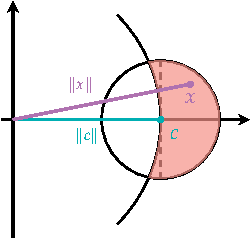
\includegraphics[width=0.5\textwidth]{figures/J-L-lemma/stein.pdf}
    \caption{高维空间中的采样点}
    \label{fig:circle-sample}
\end{figure}

现在,我们回到最早的估计问题,我们把$\mu$看作是圆心$c$,而随机采样的点就看作是样本点. 上面的概率不等式意味着,随着维数变高,朴素估计量$x$与真正的$\mu$之间的的差距会越来越大. 不仅如此,朴素估计量对$\mu$的估计会偏大. 

直觉上,要想更加精确估计$\mu$,我们需要比样本点$x$更接近圆心$c$. 仔细观察 \eqref{eq:James-Stein-estimation},James-Stein估计量的确是这样做的. 下面,我们详细介绍这一估计量的几何推导. 

由于坐标系的选取是随意的,可以设一条坐标轴和$\mu$的方向相同,其他$n-2$根坐标轴方向随意,但正交. 在新坐标系下,$\mu = (\norm{\mu},0,\dots,0)^\t$. 

设样本是$x=(x_1,x_2,\dots,x_n)^\t$. 损失函数可以被分解成两个部分的和:
\begin{equation}
    \ell=(x_1-\norm{\mu})^2+\sum_{i=2}^nx_i^2. \label{eq:loss-decomposition}
\end{equation}
令
\[\rho = \sqrt{\sum_{i=2}^n x_i^2}.\]
因为$x$是分量相互独立的Gauss向量,坐标轴旋转不改变分量之间的独立性,因此$\rho$服从自由度为$n-1$的$\chi$分布(可参见\Cref{sec:multivariate-normal}). 

假设样本点恰好满足$x_1=\norm{\mu}$,而$x_i$以概率$1$都不为$0$,可以画出\Cref{fig:triangle}. 
\begin{figure}[ht]
    \centering
    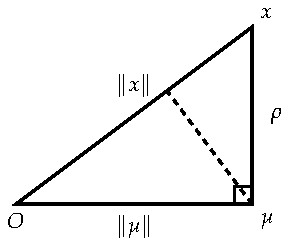
\includegraphics[width=0.5\textwidth]{figures/J-L-lemma/triangle.pdf}
    \caption{$x$与$\mu$形成的直角三角形}
    \label{fig:triangle}
\end{figure}

如果我们直接用样本点$x$作为估计量$\hat\mu$,那么我们产生的偏差在于直边上,因此会有$\rho^2$的损失. 现在,我们尝试移动$\hat\mu$,来减少损失. 

我们除了样本点$x$和原点$O$之外,其他任何信息都没有. 因此,盲目的移动反而会带来更大的损失. 结合前面的讨论,我们想要将$\hat\mu$靠近原点,因此,一个合理的办法就是沿着斜边$Ox$向原点移动. 

根据直角三角形的性质,当$\hat\mu-\mu$与斜边垂直的时候,损失最小. 我们来推导$\hat\mu$的表达式. 设$\hat\mu=\alpha x$. 根据三角形相似的原理,我们有
\begin{align*}
    &\frac{|O\hat\mu|}{|O\mu|}= \frac{|O\mu|}{|Ox|},\\
    \iff&\frac{\alpha\norm{x}}{\norm{\mu}}=\frac{\norm{\mu}}{\norm{x}}\\
    \iff&\alpha = \frac{\norm{\mu}^2}{\norm{x}^2}=1-\frac{\rho^2}{\norm{x}^2}.
\end{align*}

因此,新的估计量是
\[\hat\mu = \left(1-\frac{\rho^2}{\norm{x}^2}\right)x=\left(1-\frac{\rho^2}{x_1^2+x_2^2+\dots+x_n^2}\right)x.\]

然而,这一新估计量是不可计算的:因为我们只知道$O$和旋转之前的$x$,所以我们没有办法计算$\rho$. 为了得到James-Stein估计量,我们用一些数字特征来代替$\rho$. 对于自由度为$k>1$的$\chi$分布,其众数是$\sqrt{k-1}$(见习题 \ref{exercise:chi-mode}). 用众数来代替$\rho$,就得到了James-Stein估计量. 

最后,我们给出一些关于Stein悖论的讨论. 

\begin{itemize}
    \item 存在比James-Stein估计量更好的估计量. 直观上,当样本$x$过于靠近原点的时候,$\norm{x}$接近零,因此James-Stein估计量会穿过原点,往反方向跑到很远地方. 这自然会带来很大的损失. 因此,修正这一行为可以得到更好的估计量,比如
    \[\hat\mu=\ReLU\left(1-\frac{n-2}{x_1^2+x_2^2+\dots+x_n^2}\right)x,\]
    其中
    \[\ReLU(x)=\begin{cases}
        x, & x>0,\\
        0, & x\leq 0.
    \end{cases}\]
    \item 我们也可以从偏差-方差权衡的角度来理解James-Stein估计量. “距离”这一概念,在代数上,可以做如下分解:
    \begin{align*}
    \E\left[(\hat{\mu}-\mu)^2\right] &= \var \left[\hat{\mu}-\mu\right] + (\E\left[\hat{\mu}-\mu\right])^2 \\
    &= \var [\hat{\mu}] + (\E\left[\hat{\mu}-\mu\right])^2.
    \end{align*}
    前半部分是方差(距离差的平方的期望),后半部分是偏差(距离差的期望的平方). 朴素估计是无偏差估计,但会引入很大的方差. 通过适当引入偏差可能会减小方差,从而减小总体的预测误差,这就是James-Stein估计量的原理. 
    
    不过,如果你仔细观察会发现,实际上 \eqref{eq:loss-decomposition} 的第一项就是方差,第二项是偏差. 因而,偏差-方差权衡(代数直观)和几何直观其实在说同一件事情. 

    \item 为什么James-Stein估计量在一维和二维空间中不起效?Lawrence Brown证明了如下的定理:$n$维空间中的朴素估计量是可接受的当且仅当$n$维空间中的简单对称随机游走以概率$1$无限次返回原点. 这一惊人的联系揭示了这一问题的答案. 
    
    一维和二维空间中的随机游走都会以概率$1$无限次返回原点,因此朴素估计量是可接受的,所以我们不可能找到更好的估计量. 而更高维的空间中,随机游走以概率$1$无限次返回原点的概率是$0$,因此朴素估计量是不可接受的,所以James-Stein估计量就起效了!

    \item Stein悖论不意味着“中国茶叶的价格可以帮助预测墨尔本的降雨概率”. 尽管我们总是可以把毫不相关的随机事件捆绑在一起,然后利用James-Stein估计量减少总体的预测误差,但是这不意味着对其中任何一个事件的预测会更准确. 
\end{itemize}

\subsection{为什么我们要正则化?远有潜龙,勿用}

在前两节中,我们用了一些简单、理想化的模型说明了高维空间的一些奇异性质. 尽管真实的机器学习问题远比这些讨论要复杂,但他们所带来的启示不容忽视. 

在机器学习中,我们可以把问题都归结为参数估计问题. 虽然参数空间的“原点”看起来并没有什么不同,但原点这一概念本身确实带着人类先验的知识. 例如,如果一个神经网络的所有参数都是零,无论输入是什么,它都会输出全零. 同样,在Stein悖论中,靠近原点就是会产生更好的估计量. 

在机器学习中,我们同样有偏好“原点”的倾向,例如使用$L^2$正则化这样的技术可以使模型变得更简单,因此不太可能过拟合. 本节的内容通过极端的例子展示了正则化背后的原理:在高维空间中,离原点较远的地方体积远大于靠近原点的地方. 因此,在高维空间中,向原点收缩一点就能减少大量的参数空间. 

换句话说,对于一个大型机器学习模型来说,过拟合的方式远多于欠拟合的方式,所以我们倾向于让模型更偏向于欠拟合:欠拟合只会带来少部分问题,而过拟合带来的是数不胜数、千奇百怪的问题. 

模型越远离原点,它的行为就越难以控制和解释. 高维几何与Stein悖论给我们的启示是,远离原点就会有危险,而在高维空间中,稍微远离原点就会引入大量危险. 化用《周易》的一句话:
\begin{quotation}
    \textit{“远有潜龙,勿用. ”}\footnote{原句出自《周易·乾卦》,“初九:潜龙勿用. ”孔子对这句话的解释是如果身居下位,时机还没有成熟,应当像潜藏的龙一样不要施展你的才干. 这里,复杂的、远离原点模型就像是潜龙,隐藏着巨大的力量,但是现在人类对他们的理解还远远不够,因此我们应当保持谨慎,不要轻易使用. }
\end{quotation}

\section{集中不等式}

我们在前一节中阐述了高维空间中怪诞反直觉的性质. 从本节开始,我们将阐述高维空间中随机变量的另一重属性:集中不等式. 集中不等式说明的是,尽管整个空间非常庞大、难以理解,但如果随机变量具有某些性质,那么它们的取值就会集中在某个非常小的区域内,因而并没有我们所设想的那么复杂. 利用这一原理,我们可以将非常高维的数据压缩到一个较为低维的空间中,从而可以驾驭他们. 

接下来,我们先做一些准备工作,更详细的讨论参见\Cref{chap:prob}. 我们先引入示性函数的概念.
\begin{definition}[示性函数]\label{def:indicator-function}
    对事件$A$,定义$A$的\textbf{示性函数}为一个从样本空间$\Omega$到$\R$的随机变量:
\begin{equation*}
    I(A)(\omega) := 
    \begin{cases}
        1,& \omega \in A. \\
        0,& \omega \notin A.
    \end{cases}
\end{equation*}
\end{definition}

从定义就可以得到如下基本性质:
\begin{proposition}\label{prop:indicator-function}
    设$A, B$是两个事件,则
    \begin{enumerate}
        \item $I(AB) = I(A) I(B)$.
        \item $I(A)^2 = I(A)$.
        \item $I(A\cup B) = I(A) +I(B) - I(AB) $.
    \end{enumerate}
\end{proposition}
\begin{proof}
    这里只作为一个示意,证明第三点,其他都类似. 我们需要证明,对任意样本点$\omega\in\Omega$,我们有
    \[
        I(A\cup B)(\omega) = I(A)(\omega) + I(B)(\omega) - I(AB)(\omega).
    \]
    假设$\omega\in A\cup B$,那么左边等于$1$. 我们分类讨论:
    \begin{itemize}
        \item 如果$\omega\in A$,那么右边第一项为$1$.
        \begin{itemize}
            \item 如果$\omega\in B$,那么右边第二项为$1$. 此时自然也有$\omega\in AB$,所以右边第三项为$1$,因此右边等于$1$,等于左边. 
            \item 如果$\omega\notin B$,那么右边第二项为$0$. 此时自然也有$\omega\notin AB$,所以右边第三项为$0$,因此右边等于$1$,等于左边. 
        \end{itemize}
        \item 如果$\omega\notin A$,那么右边第一项为$0$. 此时必须有$\omega\in B$,所以右边第二项为$1$. 但是此时自然也有$\omega\notin AB$,所以右边第三项为$0$,因此右边等于$1$,等于左边. 
    \end{itemize}
    如果$\omega\notin A\cup B$,讨论类似,这里不再赘述. 
\end{proof}

示性函数之所以重要,是因为它联系了期望与概率. 我们先来看一个显然的命题:
\begin{proposition}\label{prop:expectation-of-indicator-function}
    设$A$是一个事件,则
    \[
        \E[I(A)] = \Pr(A).
    \]
\end{proposition}

示性函数可以把对概率的计算变成对期望的计算. 回忆期望的线性性(见\Cref{prop:expectation-property}):设$a,b\in\R$,$X,Y$是有期望的随机变量,那么成立
\[\E(aX+bY)=a\E(X)+b\E(Y).\]
利用期望的线性性,示性函数可以导出很多概率恒等式与不等式. 例如:容斥公式
\begin{align*}
    \Pr(A\cup B) &= \E[I(A\cup B)] = \E[I(A) + I(B) - I(AB)] \\
    &= \E[I(A)] +  \E[I(B)] -  \E[I(AB)]\\
    &= \Pr(A) + \Pr(B) - \Pr(AB).
\end{align*}

对于概率论以及机器学习理论来说,下面的这个不等式非常重要:

\begin{theorem}[Markov不等式]\label{thm:markov-inequality}
    如果$X$是非负有期望的随机变量,$a>0$,那么
        \[
            \Pr(X\geq a) \leq \frac{\E[X]}{a}.
        \]
\end{theorem}

\begin{proof}
直接利用示性函数,我们有:
    \begin{align*}
        \E[X] = &\E[X I(X\geq a)+X I(X<a)]\\
        =&\E[\underbrace{X I(X\geq a)}_{\geq aI(X\geq a)}]+\E[\underbrace{XI(X<a)}_{\geq 0}]\\
        \geq& a\E[I(X\geq a)]=a\Pr(X\geq a).
    \end{align*}
\end{proof}

注意,为了使得证明有效,我们必须要假设上面的推导中出现的期望都是存在的,当然这实际上很容易验证. 为了避免不必要的技术细节,在后面的所有证明以及推导中,我们都会默认写出来的期望是存在的,不再赘述. 

我们利用Markov不等式可以直接得到以下结果. 
\begin{corollary}[Chebyshev不等式]\label{cor:chebyshev-inequality}
设$X$是任意有方差的随机变量,那么对任意$a>0$,成立
    \[
        \Pr(|X - \E[X]| \geq a) \leq \frac{\var(X)}{a^2}.
    \]
\end{corollary}
\begin{proof}
设$Y=(X-\E[X])^2$,$t=a^2$,那么$Y$是非负随机变量,且$\E[Y]=\var(X)$,于是由Markov不等式,我们有
\begin{align*}
    \Pr(|X - \E[X]| \geq a) &= \Pr(|X - \E[X]|^2 \geq a^2) \\
    &=\Pr(Y \geq t) \\
    &\leq \frac{\E[Y]}{t}=\frac{\var(X)}{a^2}.
\end{align*}
\end{proof}

Chebyshev不等式告诉我们采样到偏离其期望的概率有一个上界. 像这样利用矩(即$\E[f(X)]$)来估计概率上界的方法被称为\textit{矩法}. 

实际上,很多情况下,偏离期望是非常小概率的事件,远小于上面的估计值. 为了得到更精确的上界,我们需要一些技巧. 考虑任意随机变量$X$,对$\lambda >0$,
\[
X\geq a \iff \lambda X \geq \lambda a \iff \e^{\lambda X} \geq \e^{\lambda a}.
\]
由Markov不等式(如何得到?),
\[
\Pr(X\geq a) = \Pr\left(\e^{\lambda X} \geq \e^{\lambda a}\right) \leq \e^{- \lambda a}\cdot \E\left[\e^{\lambda X}\right]. 
\]
注意到这个不等式应该对任意$\lambda > 0$ 成立,所以
\[
\Pr(X\geq a) \leq \inf_{\lambda >0} \e^{- \lambda a}\cdot \E \left[\e^{\lambda X}\right].
\]

以上方法可以得到概率更精确的上界. 这样用指数进行推导的方法称为\textit{指数矩}或\textit{Cramér-Chernoff方法}. 

利用指数矩,我们可以更加精确地研究Chebyshev不等式中随机变量所表现出来的性质,这种性质被称为概率的\textit{集中性}. 我们可以用\textit{集中不等式}来刻画这样的性质. 这样的不等式描述随机变量$X$有多大概率偏离某个值$\mu$多少值($t$),它表现为
\[
\Pr(| X - \mu| \geq t) \leq \text{ 小量}.
\]
通常来说,$\mu$是随机变量的期望或者中位数,在这本书中,只会讨论关于期望的集中性. 我们可以看到Chebyshev不等式就是一种特殊的集中不等式,但是它的界太松. 利用指数矩,我们将证明界更紧的Hoeffding不等式和Chernoff不等式. 

\begin{theorem}[Hoeffding 不等式]\label{thm:hoeffding-inequality}
    设$X_1, \dots, X_n$相互独立且服从对称Bernoulli分布,即$X_i$满足$\Pr(X_i=1)=1-\Pr(X_i=-1)=1/2$. 考虑向量$a = (a_1, \dots, a_n) \in \R^n$,对任意$t\geq0$,我们有
    \[
        \Pr\left(\sum_{i=1}^n a_i X_i \geq t\right)\leq \exp \left( - \frac{t^2}{2\norm{a}^2_2}\right).
    \]
\end{theorem}
\begin{proof}
由指数矩,我们有
\[
\begin{aligned}
    \Pr\left(\sum_{i=1}^n a_i X_i \geq t\right) &= \Pr\left(\exp\left(\lambda \sum_{i=1}^n a_i X_i\right) \geq \exp\left(\lambda t\right)\right) \\
    &\leq \e^{-\lambda t} \E \left[\exp\left(\lambda \sum_{i=1}^n a_i X_i\right)\right]\\
    &=  \e^{-\lambda t}\prod_{i=1}^n \E\left[\exp\left(\lambda a_i X_i\right)\right].
\end{aligned}
\]
这个不等式对任意$\lambda > 0$都成立. 

利用$X_1, \dots, X_n$服从对称Bernoulli分布,得到(习题 \ref{exercise:expoential-moment}):
\begin{equation}
\e^{-\lambda t}\prod_{i} \E\left[\exp\left(\lambda a_i X_i\right)\right]\leq\exp \left(-\lambda t + \frac{\lambda^2}{2} \sum_{i} a_i^2\right).\label{eq:exponential-moment}
\end{equation}
由于这一不等式对任意$\lambda > 0$都成立,根据二次函数的性质,取$\lambda = t / \sum_i a_i^2$,可得
\[
\begin{aligned}
    \inf_{\lambda>0}\exp \left(-\lambda t + \frac{\lambda^2}{2} \sum_{i} a_i^2\right) &=\exp\left( -\frac{t}{\sum_i a_i^2} t + \frac12 \left(\frac{t}{\sum_i a_i^2}\right)^2 \sum_{i} a_i^2\right) \\
    &= \exp \left( - \frac{t^2}{2\norm{a}_2^2}\right).
\end{aligned}
\]
\end{proof}

利用相同的证明技巧,我们可以证明一般形式的Hoeffding不等式(见习题 \ref{exercise:hoeffding-inequality-general}).

\begin{theorem}[Hoeffding 不等式,一般情形]\label{thm:hoeffding-inequality-general}
    设$X_1, \dots, X_n$是相互独立的随机变量,对任意$i$都成立$X_i \in [m_i, M_i]$. 那么对任意$t\geq0$,我们有
    \[
        \Pr\left(\sum_{i=1}^n (X_i - \E [X_i]) \geq t\right) \leq \exp \left( - \frac{2t^2}{\sum_{i=1}^n (M_i - m_i)^2}\right).
    \]
\end{theorem}

下面我们介绍 Chernoff 不等式. 
\begin{theorem}[Chernoff 不等式]\label{thm:chernoff-inequality}
    设$X_1, \dots, X_n$是相互独立的随机变量,分别服从于参数为$p_1, \dots, p_n$的Bernoulli分布.  记$\sum_{i=1}^n X_i$的期望为$\mu = \sum_{i=1}^n p_i$,对于任意$t > \mu$,我们有
    \[
        \Pr\left( \sum_{i=1}^n X_i \geq t\right) \leq \e^{-\mu} \left(\frac{\e\mu}{t}\right)^t.  
    \]
    这里$e$是自然对数的底数.
\end{theorem}

\begin{proof}
和证明Hoeffding 不等式的第一步相同,我们先利用指数矩,对任意$\lambda > 0$有
    \[
    \begin{aligned}
        \Pr\left( \sum_{i=1}^n X_i \geq t\right) &\leq \e^{-\lambda t}\prod_{i=1}^n \E\left[\exp (\lambda X_i)\right].
    \end{aligned}
    \]
然后,将$\prod_{i=1}^n\E[\exp (\lambda X_i)]$进一步放缩:
    \[
    \begin{aligned}
        \prod_{i=1}^n \E \left[\exp (\lambda X_i)\right]&= \prod_{i=1}^n \left(\e^\lambda p_i + (1 - p_i) \right) \\
         &\leq \prod_{i=1}^n \exp\left((\e^\lambda -1)p_i \right). \\
    \end{aligned}
    \]
因此
    \[
    \begin{aligned}
        \Pr\left( \sum_{i=1}^n X_i \geq t\right) &\leq \e^{-\lambda t}\prod_{i=1}^n \exp\left((\e^\lambda -1)p_i \right) \\
        &= \e^{-\lambda t} \exp\left((\e^\lambda -1)\sum_{i=1}^n p_i \right)\\
        &=\exp\left(\mu \e^\lambda -t\lambda-\mu \right).
    \end{aligned}
    \]
右边的最小值在$\lambda = \log (t/\mu)$取得,代入得到:
    \[
    \begin{aligned}
        \Pr\left( \sum_{i=1}^n X_i \geq t\right) \leq \e^{-\mu} \left(\frac{\e\mu}{t}\right)^t.
    \end{aligned}
    \]
\end{proof}

\section{J-L引理的陈述与证明}
有了上面矩法的准备,我们可以陈述并证明J-L引理了.
\begin{theorem}[Johnson-Lindenstrauss 引理]\label{thm:johnson-lindenstrauss-lemma}
给定$N$个单位向量$v_1,\dots,v_N\in\R^m$和$n >24\log N/\epsilon^2$,随机矩阵$A\in \R^{n\times m}$每个元素独立重复采样自$\Nor(0,1/n)$,$\epsilon \in (0,1)$是给定常数,那么至少有$(N-1)/N$的概率,使得对所有的$i\neq j$,都成立
    \[
        (1 - \epsilon)\norm{v_i-v_j}_2^2 <\norm{Av_i-Av_j}_2^2 < (1 + \epsilon)\norm{v_i-v_j}_2^2.
    \]
\end{theorem}

我们可以把$n$理解成降维后的维度,$Av_i$是降维后的向量. 这个引理告诉我们只要$n > 24\log N/\epsilon^2$,我们就可以用变换$A$把原本$m$维的向量映射到$n$维空间,并且保证它们相对距离的偏离不超过$\epsilon$.

通常来说,相对距离编码了很多重要的信息. 例如,如果两个人的年龄、身高、体重等属性相差很小,那么他们也应该更相似. 在这种观点下,我们可以把$A$看成一个损失率很低的压缩变换. 不严格地说,
\begin{quotation}
    \textit{塞下$N$个向量,只需要$\O(\log N)$维空间.}
\end{quotation}

值得注意的是,J-L引理中压缩空间的维数并不依赖于原始空间的维数,而只依赖于数据的数量. 因此,这对于一些抽象空间中数据的降维是非常有用的,见\Cref{sec:J-L-applications}.

下面我们开始证明J-L引理. 为了看出来证明的思路,我们第一个任务是算出压缩后$Av_i$的分布. 我们首先回忆一些正态向量的基本性质(参考\Cref{sec:multivariate-normal}). 

\begin{proposition}\label{prop:gaussian-vector}
假设$u\sim\Nor(\mu,\Sigma)$是一个$n$维正态向量,$M$是一个$m\times n$矩阵,那么$Mu$是一个$m$维正态向量,并且$Au\sim \Nor(M\mu,M\Sigma M^T)$.
\end{proposition}

利用这一个命题,很容易可以得到$Av_i$的分布:

\begin{lemma}\label{lemma:gaussian-vector}
    假设$u\in\R^m$是一个单位向量,那么$Au\sim \Nor(0,n^{-1}I_n)$.
\end{lemma}
\begin{proof}
    将$A$视作一个$mn$维的正态向量,注意到,$(Au)_i = \sum_{j=1}^m A_{ij}u_j$,所以$Au$是一个从向量$A$线性变换得到的向量. 根据\Cref{prop:gaussian-vector},$Au$是一个正态向量,只需计算它的期望和协方差矩阵. 
   
   注意到,对不同的$i$,向量$(A_{ij})_{j}$相互是独立的,所以分量$(Au)_i$相互也是独立的,因此只需要计算正态变量$(Au)_i$的期望与方差. 其期望为$\sum_{j=1}^m 0\cdot u_j = 0$,方差为
   \[\sum_{j=1}^m \left(\frac{1}{n}\cdot u_j^2\right) = \frac{1}{n}.\] 
   所以$Au$的期望是$0$,协方差矩阵是$n^{-1}I_n$.
\end{proof}

然而,我们关心的其实不单单是$Av_i$的分布,更重要的其实是$Av_i-Av_j$的分布,即压缩后的向量之间的相对距离. 不过,我们并不需要做额外的什么计算,我们直接有如下结果:

\begin{lemma}\label{lemma:gaussian-vector-diff}
    向量$u=\frac{v_i-v_j}{\norm{v_i-v_j}_2}$是一个单位向量,因此$Au\sim \Nor(0,n^{-1}I_n)$.
\end{lemma}

J-L引理实际上在说,$\norm{Au}_2$偏离$1$的一定程度的概率是非常小的. 于是,为了证明J-L引理,我们最重要的任务是给出$Au$这样向量模长的集中不等式:
\begin{lemma}[单位模引理]\label{lemma:unit-mod-lemma}
    设 $u\sim \Nor(0,n^{-1}I_n)$,$\epsilon \in (0,1 )$是给定的常数,那么我们有
    \[
        \Pr(|\norm{u}_2^2 - 1| \geq \epsilon) \leq 2\exp \left(-\frac{\epsilon^2 n}{8}\right).
    \]
\end{lemma}
注意到$\E[\norm{u}_2^2]=n\cdot(1/n)=1$,所以这个引理在说高维空间中,如果正态向量具有单位模长平方期望,那么它的模长就会集中在单位长度附近,因此称为单位模引理.

\begin{proof}
$|\norm{u}_2^2 - 1| \geq \epsilon$发生有两种可能,$ \norm{u}_2^2 - 1 \geq \epsilon$和$ 1 - \norm{u}_2^2 \geq \epsilon$. 我们先来计算$ \norm{u}_2^2 - 1 \geq \epsilon$的概率,根据指数矩,
    \[
    \Pr\left(\norm{u}_2^2 - 1 \geq \epsilon\right) \leq \inf_{\lambda > 0} \left\{\e^{- \lambda (\epsilon + 1)} \E \left[\e^{\lambda \norm{u}_2^2}\right]\right\}. 
    \]
因为$u$的各个分量是相互独立的,所以我们可以把$\norm{u}_2^2$展开
    \[
    \E\left[\e^{\lambda \norm{u}_2^2}\right] = \E\left[\e^{\lambda \sum_i u_i^2}\right] = \E\left[\prod_i \e^{\lambda u_i^2}\right] = \prod_i \E\left[\e^{\lambda u_i^2}\right]. 
    \]
可以算得$\E\left[\e^{\lambda u_i^2}\right]= \sqrt{n/(n-2\lambda)}$(见习题 \ref{exercise:moment-of-gaussian}),所以
    \[
    \Pr\left(\norm{u}_2^2 - 1 \geq \epsilon\right) \leq \inf_{\lambda > 0} \left\{\e^{- \lambda (\epsilon + 1)} \left(\frac{n}{n-2\lambda} \right)^{n/2}\right\}. 
    \]
可以验证最小值在$\lambda = n\epsilon/(2(1+\epsilon))$处取到,代入可得
    \[
    \Pr\left(\norm{u}_2^2 - 1 \geq \epsilon\right) \leq \e^{n(\log (1+\epsilon) - \epsilon)/2} \leq \e^{-n\epsilon^2/8}. 
    \]
这里最后一个不等号使用了不等式$\log(1+\epsilon)\leq\epsilon-\epsilon^2/4$. 

计算$1 - \norm{u}_2^2 \geq \epsilon$的概率的过程和$\norm{u}_2^2 - 1 \geq \epsilon$几乎完全相同的,可以得到
    \[
    \Pr\left(1 - \norm{u}_2^2 \geq \epsilon\right) \leq \e^{n(\log (1-\epsilon) + \epsilon)/2} \leq \e^{-n\epsilon^2/8}. 
    \]
    \begin{align*}
        \Pr\left(| \norm{u}_2^2 - 1| \geq \epsilon\right) &\leq \Pr\left(\norm{u}_2^2 - 1 \geq \epsilon\right) + \Pr\left(1 - \norm{u}_2^2 \geq \epsilon\right) \\
        &\leq 2\e^{-n\epsilon^2/8}. 
    \end{align*}
\end{proof}

有了单位模引理,我们就可以很容易证明J-L引理了. 将\Cref{lemma:gaussian-vector-diff} 中的$u$带入单位模引理,得到
\[
    \Pr\left(\left|\norm{\frac{A(v_i-v_j)}{\norm{v_i-v_j}_2}}_2^2 - 1 \right| \geq \epsilon\right)\leq  2\exp \left(-\frac{\epsilon^2 n}{8}\right). 
\]
这个结论对任意$i\neq j$成立,因此遍历所有$i,j$对,可得
\[
\begin{aligned}
    \Pr\left(\exists (i,j): \left|\norm{\frac{A(v_i-v_j)}{\norm{v_i-v_j}_2}}_2^2 - 1 \right| \geq \epsilon\right)
    &\leq 2 \sum_{i\neq j} \exp \left(-\frac{\epsilon^2 n}{8}\right) \\
    &=  2  \binom{N}{2}\exp \left(-\frac{\epsilon^2 n}{8}\right). 
\end{aligned}
\]
换言之,对任意$i,j$,$\left|\norm{\frac{A(v_i-v_j)}{\norm{v_i-v_j}_2}}_2^2 - 1 \right| < \epsilon$都成立的概率不小于
\[
1 - 2  \binom{N}{2}\exp \left(-\frac{\epsilon^2 n}{8}\right) = 1 - N(N-1)\exp \left(-\frac{\epsilon^2 n}{8}\right). 
\]
代入$n > \frac{24\log N}{\epsilon^2}$,可得这一概率
\[
1 - N(N-1)\exp \left(-\frac{\epsilon^2 n}{8}\right) \geq 1 - N(N-1)N^{-3}\geq 1 - N^{-1} = \frac{N-1}{N}. 
\]

很多时候,我们关心的并不是向量间的距离,而是向量的内积(比如使用\textit{余弦度量}的时候),这时候我们可以使用内积版本的J-L的引理:
\begin{theorem}[J-L引理,内积形式]\label{thm:johnson-lindenstrauss-lemma-inner-product}
    给定$N$个单位向量$v_1,\dots,v_N\in\R^m$和$n > 24\log N/\epsilon^2$,随机矩阵$A\in \R^{n\times m}$每一个元素都独立重复采样自$\Nor(0,1/n)$,$\epsilon \in (0,1)$是给定常数,那么至少有$(N-1)/N$的概率,使得对所有的$i\neq j$,都成立
    \[
        |\langle Av_i, Av_j\rangle - \inner{v_i}{v_j}|< \epsilon.
    \]
\end{theorem}    
\begin{proof}
由原始J-L引理可知,至少有$\frac{N-1}{N}$的概率满足对于任意$i\neq j$有:
    \[
    \begin{aligned}
        &(1 - \epsilon)\norm{v_i-v_j}_2^2 < \norm{Av_i-Av_j}_2^2< (1 + \epsilon)\norm{v_i-v_j}_2^2, \\
        &(1 - \epsilon)\norm{v_i+v_j}_2^2 < \norm{Av_i+Av_j}_2^2 < (1 + \epsilon)\norm{v_i+v_j}_2^2. 
    \end{aligned}
    \]
我们将第一行乘$-1$加到第二行可以得到
    \[
        4\inner{v_i}{v_j} - 2 \epsilon (\norm{v_i}_2^2 + \norm{v_j}_2^2) <4\langle Av_i, Av_j\rangle < 4\inner{v_i}{v_j} + 2 \epsilon (\norm{v_i}_2^2 + \norm{v_j}_2^2).
    \]
因为$v_i,v_j$是单位向量,所以上式等价于$|\langle Av_i, Av_j\rangle - \inner{v_i}{v_j}|<\epsilon$. 
\end{proof}

\section{J-L引理的应用}\label{sec:J-L-applications}
J-L引理描述的是对于$N$个向量,我们可以将它们降到$\O(\log N)$维空间,并将相对距离(或内积)的误差控制在一定范围内. 
它的内容本身就和降维相关,所以最基本的应用就是直接作为降维方法. 下面我们将介绍两个具体的应用案例说明J-L引理如何指导我们在深度学习中选择合适的维度.

\begin{example}[词向量维度]\label{ex:word-vector-dimension}
在为自然语言建立深度学习模型的时候,我们面对的首要问题就是如何在计算机中表示语言. 我们以中文为例. 如果我们看一句话,中文组成的基本单元是词. 比如,这句话就可以被分解为如下成分:
\begin{quotation}
    比如 / , / 这句话 / 就 / 可以 / 被 / 分解 / 为 / 如下 / 成分
\end{quotation}
任何的中文句子都可以被这样分解,变成一个词的序列. 这一过程被称为\textit{分词}. 于是,为了表示一段中文,我们只需要能够表示所有的词. 

于是,一个基本的任务就是如何表示一个词. 词向量就是这样的一个表示方法. 它的想法很简单:我们用一个向量空间来表示所有的词,每个词对应一个向量,我们用$v(w)$来表示词$w$对应的向量. 

很多时候,这些向量之间的关系可以反映出词之间的语义关系. 例如,“男人”和“女人”之间差异应该和“国王”和“女王”之间差异是类似的. 也就是说,我们希望
\[
v(\text{男人}) - v(\text{女人}) \approx v(\text{国王}) - v(\text{女王}).
\]
这里,$\approx$表示两个向量之间比较相似. 具体来说,我们通常会用向量的内积来衡量相似度. 也就是说,给定一个词$w$,我们希望
\[
\inner{v(w)}{v(\text{男人}) - v(\text{女人})} \approx \inner{v(w)}{v(\text{国王}) - v(\text{女王})}.
\]

我们可以想象,在真实的世界中,所有的词也构成了一个抽象向量空间,以类似的方式来表示词之间的关系,但这个向量空间的维数我们完全不得而知. 对于计算机来说,我们需要选择一个确定的、压缩过的空间来表示词向量. 

为了表示这种相似性,在压缩过的词向量空间中,所有词之间的内积应该尽量保持词本身的相似度. 这正是内积形式的J-L引理(\Cref{thm:johnson-lindenstrauss-lemma-inner-product})所描述的情况. 于是,J-L引理告诉我们,$\O(\log N)$维空间足以容纳下$N$个单词,还保持了单词之间的相似性. 

到此时,我们要十分警惕“理论指导实践”这一表述的理解. J-L引理(理论)所指导的结论,成立的前提是“正态随机矩阵”,然而我们完全不清楚单词的空间是否符合这一条件. 所以,我们不能说J-L引理直接给了我们合适的词向量维度,我们只能说J-L引理给了词向量选择的一个直觉. 具体应该用多少维度的词向量,还需要实验来验证.
\end{example}

\begin{example}[多头注意力]
\textit{注意力机制}是现代深度学习架构中最核心的模块之一. 注意力机制的一种理解方式是将其看作一个键-值存储. 想象我们把数据都存储到了一个数据库中,它的存储方式是$\{k_i:v_i\}$,其中$k_i$是键,$v_i$是值,例如“性别:男”就是一种典型的键值对,其中“性别”是键,而“男”是值. 

现在,假设数据库中的所有键、值对是$\{k_i:v_i\}_{i=1}^N$,我们希望从中找到与某个查询$q$最接近的键对应的值. 在深度学习中,键、值、查询都可以按照\Cref{ex:word-vector-dimension} 的方式表示成向量. 类似地,我们可以用内积来衡量键和查询的相似度. 

假设这些查询和键的向量都处在$\R^d$中,那么注意力的计算公式为
\[
    a_j = \frac{\e^{\inner{q}{k_j}}}{\sum_{j=1}^N \e^{\inner{q}{k_j}}}.
\]
换言之,我们把相似性转化为了概率分布,相似度越高的键,被选中的概率越大. 我们把$d$成为\textit{注意力头大小},在很多深度学习框架中,它被记为 \verb#head_size#.

在很多场景下,一个数据库只能查询一种键-值对的关系,对于一些复杂的问题,我们可能需要查询多种不同的键-值对. 例如,对于中文来说,两个词的意思是否相近可以形成一个数据库,而两个词的词性是否相近又可以形成另一个数据库. 因此,我们需要多个注意力机制来查询不同的数据库,这就是\textit{多头注意力}.

在简化的场景下,我们可以假设所有数据库里的$k_i:v_i$对都是一致的,只是查询$q_i$不同. 那么,多头注意力就是要计算
\[
    a_{ij} = \frac{\e^{\inner{q_i}{k_j}}}{\sum_{j=1}^N \e^{\inner{q_i}{k_j}}}.
\]

类似\Cref{ex:word-vector-dimension} 的问题,如果真实世界中$a_{ij}$是$p_{ij}$,我们应该如何选择向量维数$d$才能保证$a_{ij}$能够足够好地逼近$p_{ij}$呢?这个问题和\Cref{ex:word-vector-dimension} 是一样的.

在这个例子中,词向量的维度变成了$d$,词表大小变成了数据库中的键值对数量$N$. J-L引理告诉我们的答案依然是只需要$\O(\log N)$的空间就足以容纳下$N$个键值对,还能保持多组查询与键之间的相似性. 

更为重要的是,这个压缩空间的维度$d$和查询的数量无关. 这说明,如果有同样多的参数,头很大的单头注意力机制并不如头很小的多头注意力机制. 此外,这也说明无论多少个头,多头注意力的$d$并不需要随着头的数量增加而显著增加.

同样地,J-L引理只是给了我们一个直觉,具体的维度选择还需要实验来验证.
\end{example}

\section{习题}

\begin{enumerate}[wide,labelindent=0pt]
    \item \label{exercise:volume-surface-area} 证明\Cref{thm:volume-surface-area}. 
    \item \label{exercise:stein-paradox} 证明\Cref{thm:stein-paradox}. 
    \item \label{exercise:circle-sample} 在$\R^n$中,坐标轴上有一个球心为$c$的单位球,球内均匀随机选取一个点$x$,记$p_n=\Pr(\norm{x}>\norm{c})$. 
    \begin{enumerate}
        \item 证明:$p_2>1/2$.
        \item 证明:$\lim_{n\to\infty}p_n=1$.
    \end{enumerate}
    \item \label{exercise:chi-mode} 对于一个连续型随机变量$X$,如果$X$概率密度函数为$p(x)$,那么$X$的众数是使得$p(x)$取最大值的$x$. 证明:自由度为$k>1$的$\chi$分布,其众数是$\sqrt{k-1}$. 
    \item \label{exercise:expoential-moment} 证明 \eqref{eq:exponential-moment}. 
    \item \label{exercise:hoeffding-inequality-general} 证明\Cref{thm:hoeffding-inequality-general}. 
    \item \label{exercise:moment-of-gaussian} 证明:对于正态分布$X\sim\Nor(0,1/n)$,有
    \[\E\left[\e^{\lambda X^2}\right]=\sqrt{n/(n-2\lambda)}.\] 
\end{enumerate}

% \section{章末注记}